% ++++++++++++ Psocklasse på Pi ++++++++++++++
\subsubsection{Boundary-klasse: Psoc (Pi)}\label{sec:sw_design_psoc_pi}

Denne klasse har til formål at styre \IIC kommunikationen mellem Pi og Psoc'en. 
Psoc'en har påmonteret de 4 afstandssensorer, navngivet efter deres respektive placering på bilen, samt tachometeret til at måle hjulenes omdrejningshastighed og omsætte dette til $km/t$. 
Klassen er implementeret med \texttt{getDistance()} og \texttt{get Velocity()}-metoderne som kaldes af dataklassen som dermed kan hente dataen lageret i Psocklassens attributter. 
Klassen kører sin egen tråd, men tilgås fra dataklassens tråd, derfor er de midlertidige variabler beskyttet ved brug af \texttt{std::mutex}.

\begin{figure}[h]
\centering
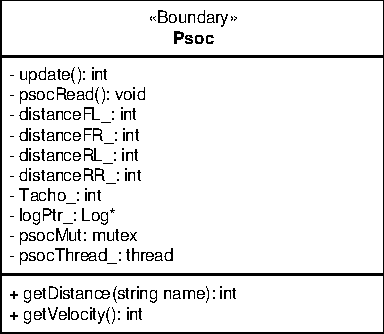
\includegraphics[]{../fig/diagrammer/bil/cd_psoc.pdf}
\caption{Klassebeskrivelse af boundary-klassen Psoc}
\label{fig:cd_psoc}
\end{figure}

\textbf{Attributter}

\begin{table}[h]
	\begin{tabularx}{\textwidth}{| Z | Z | L{10cm} |} \hline
	Navn 
		& Type  
		& Beskrivelse \\\hline
	\texttt{distanceFL\_} 	
		& \texttt{int} 		
		& Midlertidig variabel der indeholder afstanden fra forreste venstre afstandssensor.''FL''	\\\hline
	\texttt{distanceFR\_} 	
		& \texttt{int} 		
		& Midlertidig variabel der indeholder afstanden fra forreste højre afstandssensor.''FR''	\\\hline
	\texttt{distanceRL\_} 	
		& \texttt{int} 		
		& Midlertidig variabel der indeholder afstanden fra bagerste venstre afstandssensor.''RL'' 	\\\hline
	\texttt{distanceRR\_} 	
		& \texttt{int} 		
		& Midlertidig variabel der indeholder afstanden fra bagerste højre afstandssensor.''RR''	\\\hline
	\texttt{Tacho\_} 	  	
		& \texttt{int} 		
		& Midlertidig variabel der indeholder bilens hastighed										\\\hline
	\texttt{logPtr\_} 	  	
		& \texttt{log*} 	
		& Pointer til at skrive i den globale Log													\\\hline
	\texttt{PsocMut} 	  	
		& \texttt{mutex} 	
		& Mutex benyttes til at beskytte klassens attributter										\\\hline
	\texttt{psocThread\_} 	
		& \texttt{thread} 	
		& Thread benyttes til at kører klassen på en separat tråd									\\\hline
	\end{tabularx}
	\caption{Attributter for klassen Psoc}
	\label{table:attr_psoc}
\end{table}
\clearpage

\textbf{Metoder}

\begin{table}[h]
	\begin{tabularx}{\textwidth}{| L{2.5 cm} | Z |} \hline
		Prototype 	& \texttt{int getDistance(string name)} \\\hline
		Parametre 	& \texttt{name} \newline Navnet på den sensor som der skal læses fra. Kan rumme én af fire muligheder "FL", "FR", "RL" og "RR". \\\hline
		Returværdi 	& \texttt{int} \newline Seneste afstandsmåling for den pågældende sensor. Værdien er angivet i cm. \\\hline
		Beskrivelse	& Denne metode har til formål at låse attributterne (distanceFL\_ ,distanaceFR\_ ,distanaceRL\_ ,distanaceRR\_) og returnere værdierne, herefter låses attributterne automatisk op igen når metoden går ud af scope. \\\hline
	\end{tabularx}
	\caption{Metodebeskrivelse for \texttt{getDistance()}}
	\label{table:met_getdistance}
\end{table}

\begin{table}[h]
	\begin{tabularx}{\textwidth}{| L{2.5 cm} | Z |} \hline
		Prototype 	& \texttt{int getVelocity()} 	\\\hline
		Parametre 	& \texttt{void} \newline  		\\\hline
		Returværdi 	& \texttt{int}  \newline Seneste hastighedsmåling for for bilen. Værdien er angivet i $km/t$. \\\hline
		Beskrivelse	& Denne metode har til formål at låse attributten Tacho\_ og returnere den seneste værdi, herefter låses attributten automatisk op når metoden går ud af scope \\\hline	
	\end{tabularx}
	\caption{Metodebeskrivelse for  \texttt{getVelocity()}}
	\label{table:met_getvelocity}
\end{table}

\begin{table}[h]
	\begin{tabularx}{\textwidth}{| L{2.5 cm} | Z |} \hline
		Prototype 	& \texttt{int update()} 		\\\hline
		Parametre 	& \texttt{void} \newline 		\\\hline
		Returværdi 	& \texttt{int}  \newline Returnerer fejlkode hvis åbning og læsning mislykkes \\\hline
		Beskrivelse	& Denne metode har til formål at åbne \IIC-forbindelsen til PSoC'en og hente det seneste datasæt. \\\hline
	\end{tabularx}
	\caption{Metodebeskrivelse for  \texttt{update()}}
	\label{table:met_update}
\end{table}
\clearpage

\begin{table}[h]
	\begin{tabularx}{\textwidth}{| L{2.5 cm} | Z |} \hline
		Prototype 	& \texttt{int psocRead()} 		\\\hline
		Parametre 	& \texttt{void} \newline 		\\\hline
		Returværdi 	& \texttt{void} \newline 		\\\hline
		Beskrivelse	& Denne metode har til formål at kalde \texttt{update(), herefter låses attributterne og datasættet læses over heri.}\\\hline
	\end{tabularx}
	\caption{Metodebeskrivelse for  \texttt{psocRead()}}
	\label{table:met_psocRead}
\end{table}
\clearpage